\section{Technique de passation du test Tomatis}
Basé sur des sons purs et leur
 reconnaissance---ce qui permet d'objectiver la qualité de l'écoute---il
 a été créé dans les années 50 avec un
  appareil contenant un générateur de fréquences qui émet des sons
  purs s'étalant de \SIrange{125}{8000}{\Hz}, d'octave en octave, en passant par les valeurs
\SIlist{1500;3000;6000}{\Hz}, et dont l'intensité peut varier de 5 en \SI{5}{\dB}, de \SIrange{10}{100}{\dB}. 
Ceux-ci sont transmis au moyen d'une
  transmission aérienne (avec un casque) et osseuse (avec un vibrateur). Ces sons sont à identifier et à
  signaler par le patient en levant la main du côté où il l'entend. On
  débute le test avec un volume très faible en l'augmentant progressivement
  jusqu'à ce que le patient réagisse et donne une réponse. 



\begin{figure}
	\centering
	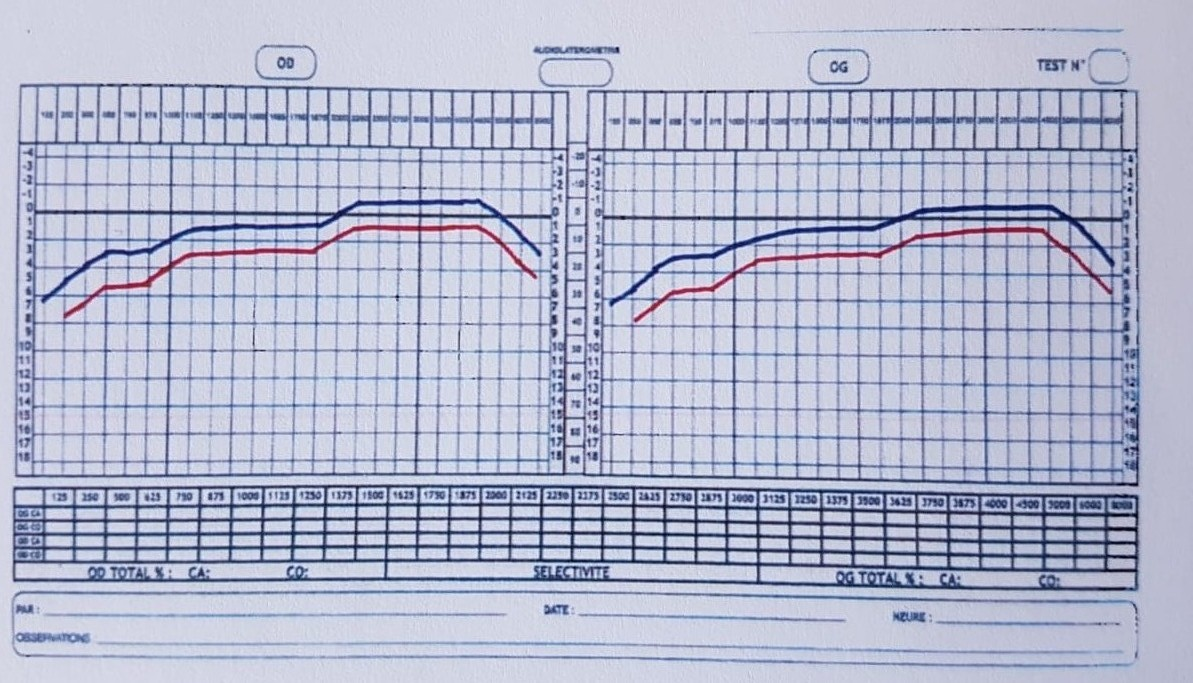
\includegraphics[width=0.7\linewidth]{images/courbeideale.jpg}
	\caption{Courbe idéale}
	\label{fig:courbeideale}
\end{figure}


Ce test a pour but de déterminer les 4 paramètres suivants : 
\begin{enumerate}
\item seuils
\item spatialisation
\item sélectivité
\item audiolatérométrie.
\end{enumerate}

\subsection{Recherche des seuils}

Il s'agit de rechercher d'une part les seuils d'audibilité
minima  avec deux types de conduction sonore, l'une \emph{aérienne} et
l'autre \emph{osseuse}.
En conduction aérienne, le son pénètre dans le conduit externe de
l'oreille par l'intermédiaire d'écouteurs. Les vibrations du tympan
parviennent à l'oreille interne qui informe le nerf auditif.

En conduction osseuse, le son pénètre à l'aide d'un
vibrateur qui vient exciter la mastoïde. Par l'intermédiaire de la
boîte crânienne, les vibrations informent le nerf auditif.

\begin{enumerate}
 	\item les seuils d'écoute sont reconnaissables par des points au niveau de 
          chaque fréquence émise et selon le volume entendu par le patient. Les points reliés créent les courbes.
 	\item le son : son pur en 20 fréquences différentes.  
 	\item le volume: dB de $-20$ à 90; un carré sur le graphique représente une différence de \SI{5}{\dB} en
 		volume 
 	\item les fréquences: 20, de 125 à 8000 Hz. 
 	\item la courbe: est le résultat des points reliés des seuils
          d'écoute; ils 
          dessinent deux courbes caractéristiques, l'une aérienne et l'autre osseuse.
          L'observation des courbes d'écoute relevées vont permettre
          de les classer selon les paramètres d'harmonie ou
          d'équilibre, ceci 
 	en comparaison avec la courbe dite idéale : on parlera
        d'équilibre ou de
 	déséquilibre, d'harmonie ou de disharmonie.
        
      \item équilibre/déséquilibre graphique:
        -entre les deux oreilles
        -entre les deux courbes aériennes et osseuses mesurées pour
        l'oreille droite et l'oreille gauche.
        Des croisements, des pics ou des échancrures, un critère
        d'écart
        entre les deux courbes répertoriées vont être des
        données qui vont permettre de
        qualifier l'écoute d'harmonieuse ou de
        déséquilibrée. 
        
 	\item Par conséquent:  transformation de l'écoute: s'il y a une modification
          graphiques des courbes, elle 
          permettra d'évaluer la modification éventuelle de l'écoute et
          et de sa transformation.
          
\end{enumerate}
 
 




\subsection{Représentation graphique}

Les résultats sont consignés sur deux grilles correspondant à la courbe
de l'oreille droite et à celle de l'oreille gauche%
\footnote{Voir fig. \ref{fig:tomatislisteningtest}. Suivant le processus d'observation habituellement appliqué en physiologie,
la place de ces deux diagrammes est inversée, la courbe droite étant
à gauche et la courbe gauche étant à droite.}.

En abscisses, on porte les fréquences de \SIrange{125}{8000}{\Hz}, et en ordonnées,
les intensités en décibels qui se lisent de haut en bas. 

Les seuils reportés sur les graphiques sont reliés entre eux et vont
dessiner deux courbes distinctes\footnote{Tomatis a volontairement décalé les étalonnages des deux courbes (aérienne
	et osseuse) pour pouvoir distinguer les différentes réponses et interpréter
	les distorsions. Lorsque l'écoute est parfaite, les
	courbes aérienne et osseuse se confondent mais pour l'analyse des
	résultats, on a déterminé des courbes parallèles, la courbe aérienne
	devant être au dessus de la courbe osseuse.}: 


\begin{figure}
	\centering
	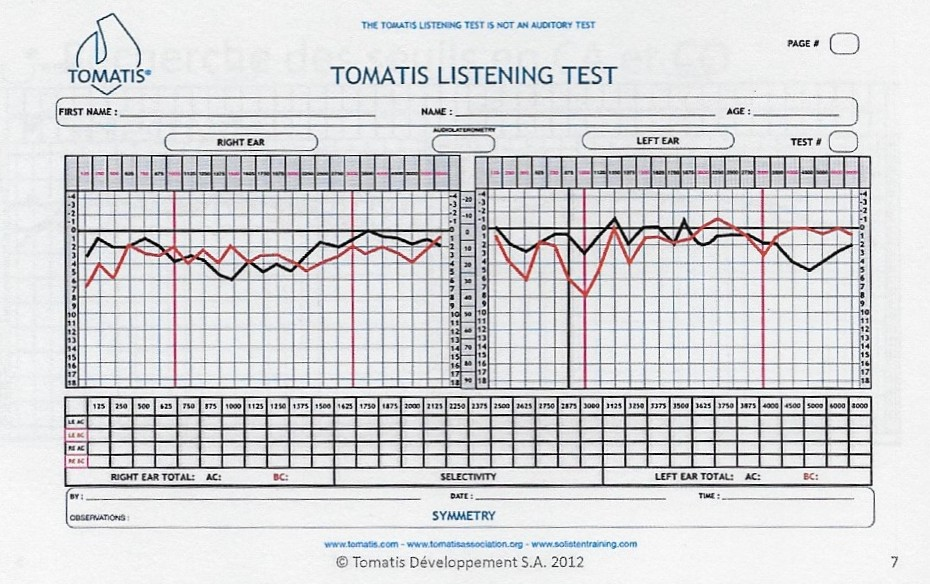
\includegraphics[width=0.7\linewidth]{images/tomatisListeningTest.jpg}
	\caption[Graphique du test d'écoute]{Graphique du test d'écoute}
	\label{fig:tomatislisteningtest}
\end{figure}

\subparagraph*{Pour notre étude, nous allons nous en tenir à la
  comparaison 
des seuils : seuil de la courbe aérienne et seuil de l'osseux des
deux oreilles, gauche et droite et leur impact sur les 3 zones.}
C'est la raison pour laquelle nous allons passer brièvement sur les
différentes techniques d'affinage de l'observation, que sont la
spatialisation, la
sélectivité et l'audiolatérométrie.

\paragraph{\'Etude de la spatialisation}


Lors de la recherche des seuils, on note en même temps le pouvoir
de l'oreille de localiser les sons dans l'espace. On recueille les
confusions ou inversions latérales de sons. Les inversions ou les
confusions de sons sont notées au niveau de chaque fréquence par un
petit trait placé au bas de chacune des grilles. La spatialisation
est un indicateur du degré d'élaboration de la latéralité auditive,
elle donne des repères sur la façon dont le patient intègre les informations
au niveau du cortex, les faisceaux homo et hétéro-latéraux devant
être fonctionnellement différenciés. 
Les erreurs de spatialisation reflètent la confusion
de l'intégration des informations au niveau du cortex et donnent une indication sur la latence et l'incertitude
dans le traitement de l'information (la manière d'appréhender le
son dans l'espace). La difficulté du sujet à fixer son
écoute relève d'une mauvaise coordination, d'un manque de confiance en soi ou
d'une mauvaise organisation des idées.



\paragraph{\'Etude de la sélectivité}

La sélectivité est la \textquote{faculté que possède une oreille de percevoir
une variation de fréquences à l'intérieur d'un spectre sonore, et
de situer le sens de cette variation}\autocite{tomatis:loreille}.
Le but est de déceler l'ouverture ou la fermeture de cette sélectivité
auditive. 
La sélectivité permet de donner des informations sur la
qualité d'écoute avec trois aspects : au niveau linguistique ( conscience
phonémique), cognitif ( fonctions exécutives) et émotionnel ( action
efférente, présence d'anxiété).
Le langage étant constitué de milliers de phonèmes, on reconnaît les possibilités auditives du patient si celui-ci  distingue au minimum la différence d'un son ``pur" d'une octave à l'autre.  


\paragraph{L'audiolatérométrie}

On recherche la latéralité du patient : droite ou gauche. La dominance
de l'oreille droite comme oreille directrice doit être manifeste car
selon ses travaux, il y a une différenciation fonctionnelle
physiologique due à la longueur des nerfs récurrents. 
Si le cerveau préfère prendre l'oreille droite comme
``directrice'', c'est que le trajet emprunté par l'oreille droite au cerveau est plus
court;
ainsi
les informations circulent plus rapidement jusqu'à l'hémisphère gauche.

Il existe donc  deux types de latéralité auditive:


\subsection{Les trois zones du test d'écoute }
 
Ainsi, après la passation du test d\textquoteright écoute, nous nous
trouvons en présence de deux grilles contenant chacune deux courbes,
en général, de deux couleurs différentes complétées par l'indication
des inversions ou confusions de sons, par des données sur la sélectivité
et en même temps par des chiffres qui correspondent à l'épreuve d'audiolatérométrie.
Les résultats du test permettront de faire une comparaison avec la
courbe idéale.
Mise en évidence de différentes zones à l\textquoteright intérieur
de chaque diagramme. 
Ces bandes sonores se répartissent en trois zones, des fréquences
graves aux aigues, de la façon suivante :
\begin{itemize}
\item Zone 1 : de 125 à 1000 Hz : les graves, la zone vestibulaire
\item Zone 2 : de 1000 à 3000 Hz : les mediums, la zone du langage
\item Zone 3 : de 3000 à 8000 Hz : les aigus, zone cochléaire
\end{itemize}



\section {Analyse et interprétation du test}

Ce sont des comparaisons graphiques des courbes. 
On considère l'allure générale des courbes, on compare leur dessin
: la forme des courbes, l' équilibre, la symétrie ; et on étudie leurs
rapports entre eux : 

courbe aérienne (CA) - courbe osseuse (CO) - rapport entre CA et CO
pour chaque oreille - rapport entre CA et CO d\textquoteright une
oreille à l'autre. si ce rapport est correct, CA est placée au-dessus
de CO sur la grille.
\subsection{Interprétation du test : }


\subparagraph{Les deux types de courbes véhiculent chacune des informations spécifiques
sur la posture d'écoute du sujet : }
\begin{itemize}
\item La conduction aérienne : traduit la vie sociale, la manière de communiquer
et de s'extérioriser
\item La conduction osseuse : traduit la vie intérieure, mode de fonctionnement
organique, d'une façon générale : liée aux tensions. C'est la courbe
de l\textquoteright auto-écoute, de l\textquoteright auto-contrôle,
de l'écoute intérieure.
\end{itemize}

\subparagraph{Les courbes donnent des informations selon leur ascendance, leur
continuité et leur similarité oreille droite/ oreille gauche.}
\begin{itemize}
\item Continuité de la courbe : Si une courbe est continue, elle définie
comme harmonieuse et ne comporte pas de pics ou de scotomes (échancrure)  qui laisseraient
supposer l'existence de nombreuse tensions.
\end{itemize}
Situées en CO, ce sont des tensions internes non exprimées : attitude
calme mais très tendue intérieurement.

Situées en CA, ce sont des tensions réelles et exprimées au quotidien
: soit somatisées, soit verbalisées ou soit manifestées sur le plan
affectif (pleurs).

\subparagraph{Les trois zones du test d'écoute : }
\begin{itemize}
\item Zone 1 : de 125 à 1000 Hz : les graves, la zone vestibulaire, élaboration
du schéma corporel, des repères temporo-spatiaux, adresse motrice,
esprit pratique.
\item Zone 2 : de 1000 à 3000 Hz : les mediums, la zone du langage, de la
verbalisation, compréhension, mémorisation, de l'intégration des lois/
des règles, esprit analytique.
\item Zone 3 : de 3000 à 8000 Hz : les aigus, zone cochléaire, de l'énergie,
de l'imagination, de l'expression, motivation, esprit synthétique.
\end{itemize}

\subparagraph{Les trois zones de fréquences du test d'écoute correspondent à des
caractéristiques précises ; et, avec l'allure des courbes, on doit
tenir compte de leurs particularités.}

Lorsqu'une zone du test d'écoute est nettement dominante et semble
traduire une caractéristique de la personnalité, on peut situer un
sujet dans un registre particulier correspondant à son tempérament.

\begin{itemize}
	\item courbe accentuée dans la zone fréquentielle des graves : tempérament
	orienté vers le corps,
	
	\item courbe accentuée dans la zone fréquentielle des médiums : tempérament
	paranoïde, attaché à la logique, la règle, le raisonnement 
	
	\item courbe accentuée dans la zone fréquentielle des aigus : tempérament
	schizoïde, reflétant une recherche de créativité. 
\end{itemize}


La simplicité de
passation pour le test d'écoute et 
 l'évaluation des indices de réception évitent toute confusion
à l'aide de réponses gestuelles.



 






